

\section{Admissible Term Structures}
\label{sec:admissible-curve}

Term-structure  construction consist  of finding  a function  $T \lra  P(t_0,T)$
given a small number market quotes $S_1,...,S_n$. For a CDS, the AIG market quotes
are given for maturities 3, 5 ,7 and 10 years :

\begin{table}[H]
  \centering
  \begin{tabular}{|c|c|c|c|c|}
    \hline
    maturity (year) & 3 & 5 & 7 & 10 \\
    \hline
    CDS spread (bp) & 58 & 54 & 52 & 49\\
    \hline
  \end{tabular}
  \caption{AIG CDS spread at Dec. 17, 2007}
\end{table}

Indeed, We  have to rely  on interpolation/calibration schemes to  construct the
curve for the  missing maturities. In previous  case the curve would  be the CDS
implied survival probability.\\
This  will lead  us  to define  what  will be  understood by  a  good yield  curve
construction.

\subsection{Market fit condition}
\label{sec:market-fit-condition}

The Term  structure function $T  \lra P(t_0,T)$ is  built from market  quotes of
standard product. Let's define some notations :
\begin{description}
\item[n] The number of product
\item[S] $=(S_1,S_2,\dots,S_n)$ The set of market quotes at $t_0$
\item[T] $=(T_1,\dots,T_n)$ the corresponding set of increasing maturities 
\item[t] $=(t_1,\dots,t_m)$ payment time grid
\end{description}

\begin{figure}[H]
  \centering
  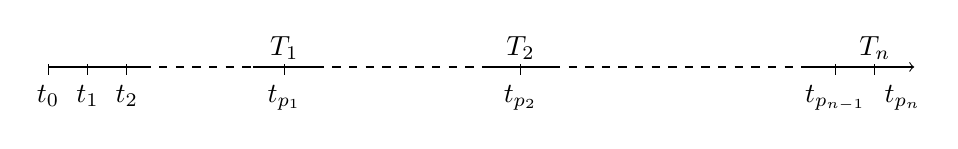
\begin{tikzpicture}
    \draw  (0 cm,1pt) -- (0 cm, -3pt) node[anchor=north] {$t_0$};
    \draw  (0.5 cm,1pt) -- (0.5 cm, -3pt) node[anchor=north] {$t_1$};
    \draw  (1 cm,1pt) -- (1 cm, -3pt) node[anchor=north] {$t_2$};
    \draw  (3 cm,1pt) -- (3 cm, -3pt) node[anchor=north] {$t_{p_1}$};
    \draw  (3 cm,1pt) -- (3 cm, -3pt) node[above=2pt] {$T_1$};
    \draw  (6 cm,1pt) -- (6 cm, -3pt) node[anchor=north] {$t_{p_2}$};
    \draw  (6 cm,1pt) -- (6 cm, -3pt) node[above=2pt] {$T_2$};

    \draw  (10 cm,1pt) -- (10 cm, -3pt) node[anchor=north] {$t_{p_{n-1}}$};
    \draw  (10.5 cm,1pt) -- (10.5 cm, -3pt) node[below right] {$t_{p_{n}}$};
    \draw  (10.5 cm,1pt) -- (10.5 cm, -3pt) node[above=2pt] {$T_n$};

    \draw (0,0) -- (1.2,0);
    \draw[dashed] (1.2,0) -- (2.8,0);
    \draw (2.6,0) -- (3.4,0);
    \draw[dashed] (3.4,0) -- (5.8,0);
    \draw (5.6,0) -- (6.4,0);
    \draw[dashed]   (6.4,0) -- (9.6,0);
    \draw[->] (9.6,0) -- (11,0);

  \end{tikzpicture}
  \caption{Time grid }
  \label{fig:3}
\end{figure}

Notice that $\forall i, \ T_i=t_{p_i}$.\\


Let $P=(P^D(t_0,t_1),\dots,P^D(t_0,t_m))$  be the  vector of  the values  of the
curve at the payment dates $t_1,\dots,t_m$:

The  market fit  condition can  be restated  as a  rectangular system  of linear
equations :
\[
A \cdot P=B
\]
where :
\begin{description}
\item[P] =$(P^D(t_0,t_1),\dots,P^D(t_0,t_m))'$ 
\item[A] is a $n \times m$ matrix
\item[B] is a $n \times 1$ matrix with positive coefficients
\item A and B only depend on current market quotes S, on standard maturities T, on payment dates t and on products characteristics.
\end{description}

\begin{example}{Credit curve based on CDS}
  for  the  CDS we  can  conclude  from \ref{eq:1}  that  under  the market  fit
  condition can be expressed as :
  \begin{eqnarray*}
    \label{eq:2}
    s_i\sum^{p_i}_{k=1}\delta_kP^D(t_0,t_k)Q(t_0,t_k)        -       (1        -
    R)P^D(t_0,T)Q(t_0,T) & \\
    + (1 - R)\int^{T_i}_{t_0}f^D(t_0,t)P^D(t_0,t)Q(t_0,t)dt & = 1 - R,\ i=1,\dots,n.
  \end{eqnarray*}
  where $f^D(t0, u)$ is the instantaneous forward (discount) rate associated with
  maturity date u.
\end{example}

In order to  get an admissible curve  $T \lra P(t_0,T)$ have to  fit some others
conditions. 

\subsection{Arbitrage-free conditions}
\label{sec:arbitr-free-cond}

\begin{de}[arbitrage-free condition]
  A credit  curve is  said to be  arbitrage-free if the  curve corresponds  to a
  well-defined default distribution  function. In other words $P$  had to verify
  the following conditions :
  \begin{itemize}
  \item $P(t_0,t_0)=1$
  \item $T\longmapsto P(t_0,T)$ is non increasing function (i.e $\exists x,y, P(t_0,x)<P(t_0,y)\&x>y$)
  \end{itemize}
\end{de}

Therefore we can have  the following inequalities, called \textit{Arbitrage-free
  inequalities} :

\begin{align*}
  P(t_0,T_1) & \leq(P(t_0,t_k)) \leq 1 & \forall k \in 1,\dots,p_1 \\
  P(t_0,T_i) &\leq(P(t_0,t_k)) \leq P(t_0,T_{i-1}) & \forall k \in [p_{i-1}+1
  , p_i-1 ]\\
\end{align*}

A.Cousin had demonstrate the following proposition :
\begin{prop}
  Assume that, at  time $t_0$, quoted fair spreads  $S_1,\dots,S_n$ are reliable
  for  standard  CDS  maturities  $T_1<\dots<T_n.$  For  any  $i=1,\dots,n$  the
  survival  probability $Q(t_0,T_i)$  associated  with  a market-compatible  and
  arbitrage-free credit curve is such that:
  \[
  Q_{min}(t_0,T_i) \leq Q(t_0,T_i) \leq Q_{max}(t_0,T_i)
  \]
  where :

  \begin{eqnarray*}
    Q_{max}(t_0,T_i) & =\frac
    {1 - R - \sum^{i - 1}_{k=1}( (1 - R) M_k + S_i N_k) Q(t_0,T_{k})}
    {P^D(t_0,T_{i - 1})(1 - R) + S_i(N_i + \delta_{p_i}P^D(t_0,T_i))}\\
    Q_{min}(t_0,T_i) &  =\frac{1 - R  - \sum^i_{k=1}  ( (1 -  R) M_k +  S_i N_k)
      Q(t_0,T_{k -1})}{P^D(t_0,T_{i})(1 - R + S_i \delta_{p_i})}\\
  \end{eqnarray*}

with :
\begin{itemize}
\item $p_0=1$, $T_0=t_0$ and $P^D(t_0,T_0)=Q(t_0,t_0)=1$
\item $\forall  i \in 1,\dots,n,\ M_i=P^D(t_0,T_{i-1})-P^D(t_0,T_i)\  and\ N_i =
  \sum^{p_i-1}_{k=p_{i-1}} \delta_k P^D(t_0,t_k)$ 
\end{itemize}
\end{prop}

this bounds can be computed recursively. Knowing that :



Will have a series of decreasing
rectangles in wich every cds credit curve should cross.
\begin{figure}[H]
  \centering
  \includegraphics[width=0.8\textwidth]{Tunnel_implied_survival_proba.eps}
  \caption{\it Union of decreasing rectangles for CDS Spreads : R=40\% and $P^D(t_0,t) = \exp(-3\%(t-t_0))$}
\end{figure}

\subsection{Application on AIG CDS data spreads}
\label{sec:application-aig-cds}

\quad If the assumption arbitrage-free is not verified the previous results will not
be relevant. Indeed we  see this phenomenon when we tried  to apply the previous
bounds  over  the  data  provided  by  {\it AIG  (France)}.  We  note  that  the
arbitrage-free inequalities where no longer verified. \\

\begin{figure}[H]
  \label{fig:5}
  \centering
  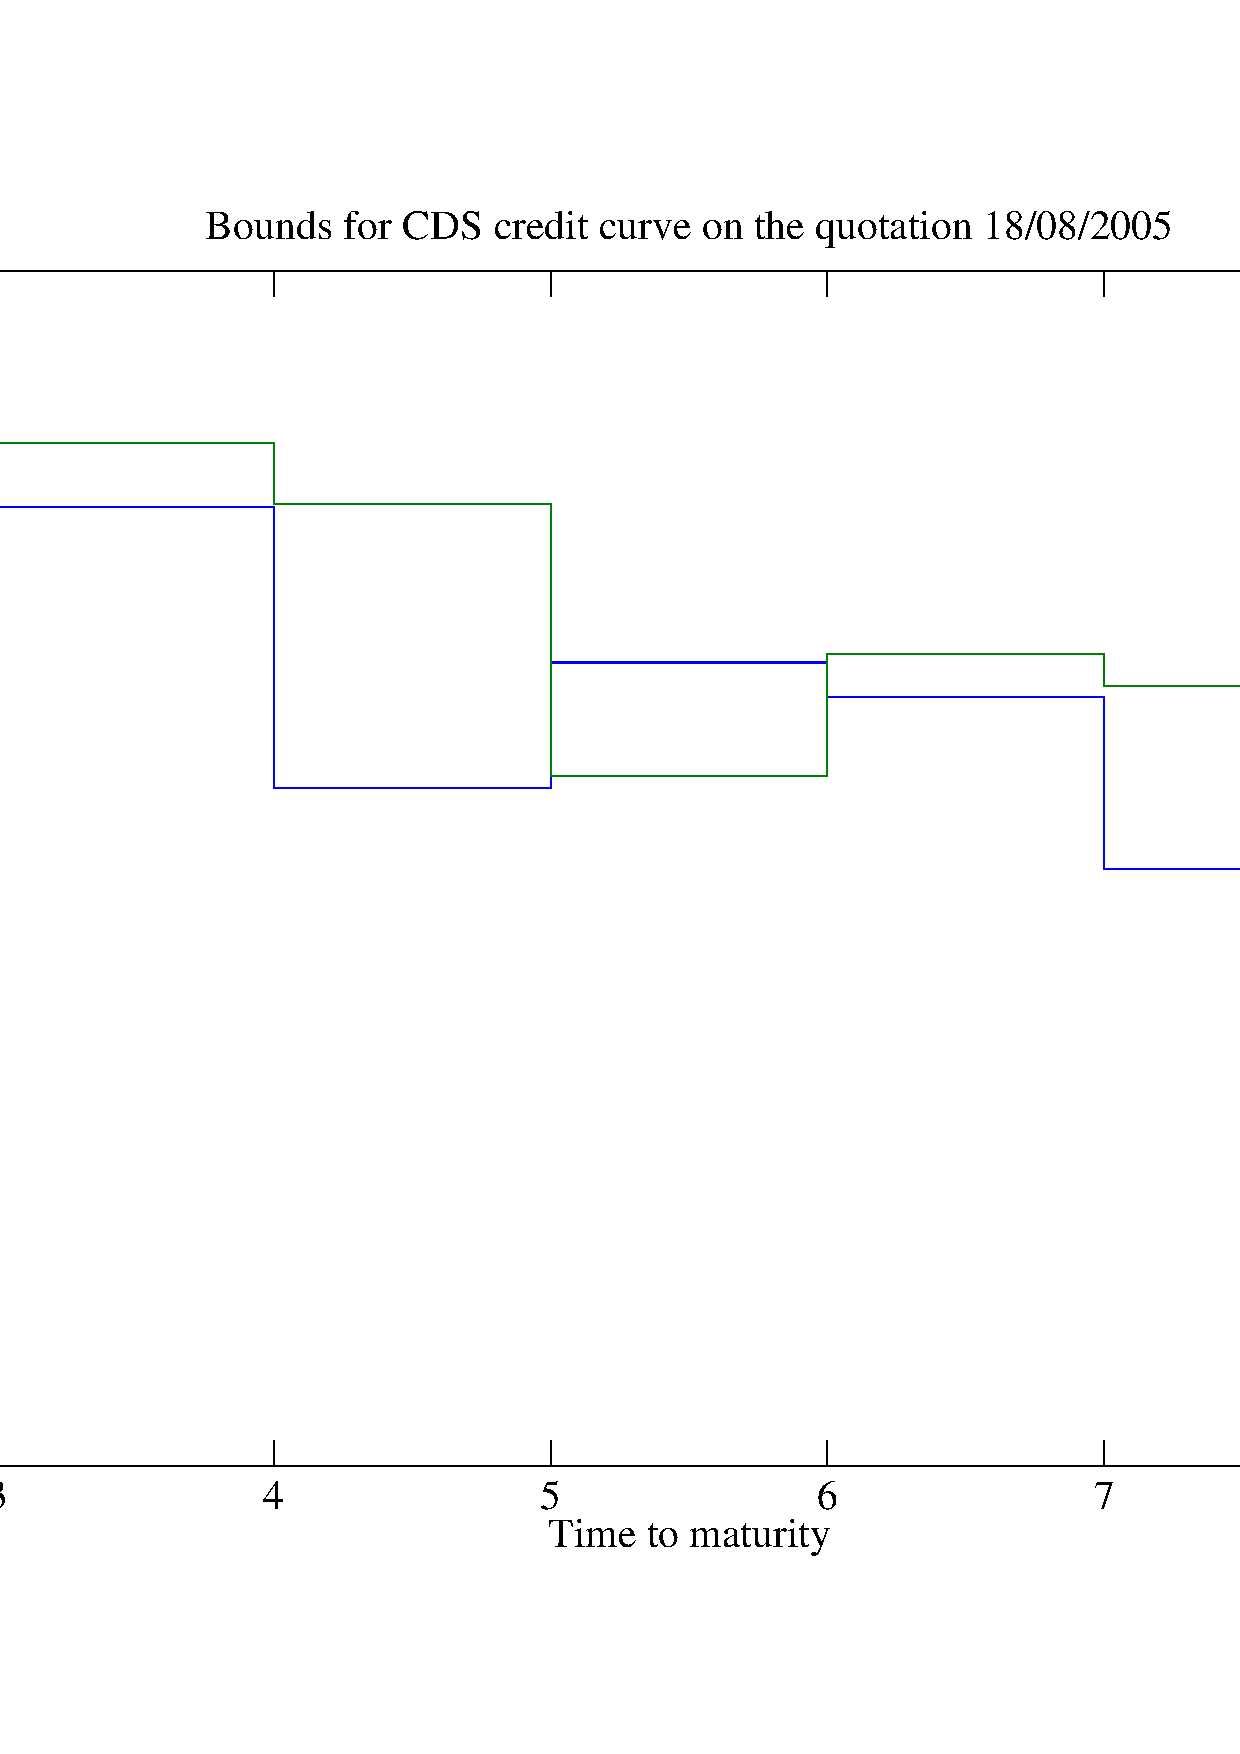
\includegraphics[width=0.7\textwidth]{cotation-18-08-2005.pdf}
  \caption{Credit curve among 18/08/2005 -  28/09/2007}
\end{figure}

It   means    that   the    market   since   18/08/2005    contained   arbitrage
opportunities.  Indeed  between  18/08/2005   -  28/09/2007  the  market  wasn't
complete.
 
\begin{figure}[H]
  \centering
  \includegraphics[width=0.8\textwidth]{cotation27-11-2007.pdf}
  \caption{Credit curve since 28/09/2007 : here in 27/11/2007}
\end{figure}


